\paragraph{Sơ đồ tuần tự luồng Đặt lại / Đổi Mật khẩu}

Luồng nghiệp vụ này mô tả
quá trình cập nhật trực tiếp mật khẩu mới của người dùng lên hệ thống bằng Access Token hợp lệ sau khi người dùng đã đi qua callback khôi phục và bước xác thực MFA.

\begin{figure}[H]
\centering
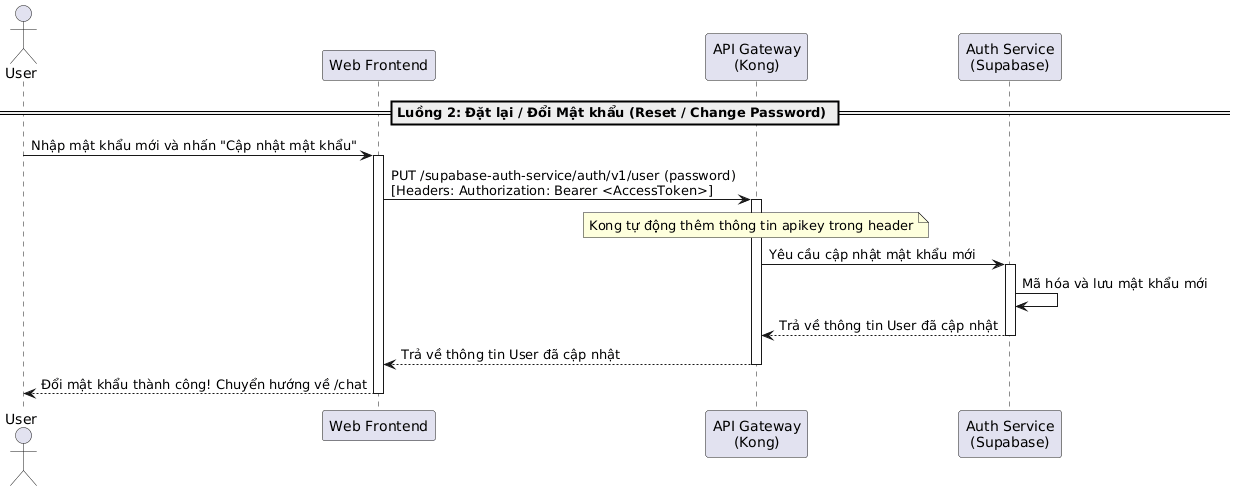
\includegraphics[scale = 0.2]{contents/Sequence/UML-Sequence-UserResetChangePassword.png}
\caption{Sơ đồ tuần tự luồng Đặt lại / Đổi Mật khẩu}
\end{figure}

\subparagraph{Các thành phần tham gia}

\begin{table}[H]
\centering
\renewcommand{\arraystretch}{1.3}

\begin{tabular}{|l|l|p{5cm}|}
\hline
\textbf{Thành phần} & \textbf{Phân loại} & \textbf{Vai trò trong hệ thống} \\ \hline
User & Actor & Người dùng thực hiện đặt lại mật khẩu mới. \\ \hline
Web Frontend & Component & Giao diện web Next.js. \\ \hline %%%% Component & Giao diện Next.js thu nhận mật khẩu mới và gửi yêu cầu đổi mật khẩu. \\ \hline
API Gateway (Kong) & Component & Cổng API chuyển tiếp các yêu cầu API. \\ \hline %%%% Component & Định tuyến yêu cầu cập nhật thông tin người dùng. \\ \hline
Auth Service (Supabase) & Microservice & Dịch vụ Supabase Auth xác thực phiên, thực hiện mã hóa và lưu mật khẩu mới. \\ \hline
\end{tabular}
\caption{Các thành phần tham gia luồng Đặt lại / Đổi Mật khẩu}
\end{table}

\subparagraph{Mô tả tổng quan}

\begin{itemize}
\item \textbf{Nhập mật khẩu mới:} Tại màn hình đổi mật khẩu, người dùng điền mật khẩu mới muốn thiết lập.
\item \textbf{Gửi yêu cầu đổi mật khẩu:} Giao diện gửi yêu cầu cập nhật mật khẩu mới qua cổng kết nối tới dịch vụ chứng thực kèm theo mã đăng nhập hợp lệ trong thông tin gửi đi.
\item \textbf{Mã hóa và lưu trữ:} Dịch vụ chứng thực kiểm tra tính hợp lệ của phiên đăng nhập, tiến hành mã hóa mật khẩu mới và lưu trữ vào cơ sở dữ liệu, sau đó trả về kết quả cập nhật thành công để giao diện chuyển hướng người dùng vào màn hình trò chuyện chính.
\end{itemize}
